% FILE: figures/axes_thresholds.tex
% Axes and threshold geometry of continua

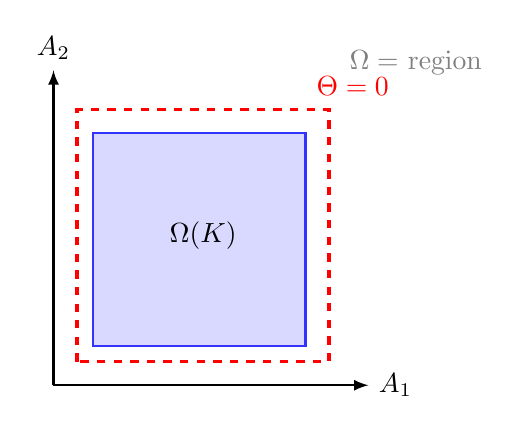
\begin{tikzpicture}[>=latex,thick]

% Axes
\draw[->] (0,0) -- (4,0) node[right] {$A_1$};
\draw[->] (0,0) -- (0,4) node[above] {$A_2$};

% State region Omega
\filldraw[fill=blue!15, draw=blue!80] (0.5,0.5) rectangle (3.2,3.2);
\node at (1.9,1.9) {$\Omega(K)$};

% Threshold boundary
\draw[red, very thick, dashed] (0.3,0.3) rectangle (3.5,3.5);
\node[red] at (3.8,3.8) {$\Theta = 0$};

% Death zone
\node[gray] at (4.6,4.1) {$\Omega = \varnothing$ region};

\end{tikzpicture}
